\section{Bayes Theorem}
\subsection*{Temporal Inferrence}
Given $\mathbf{G}$: \\
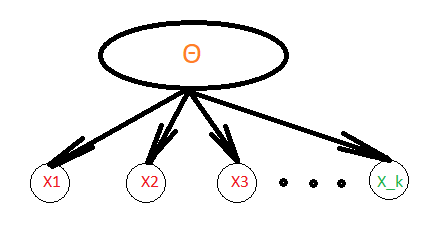
\includegraphics[width=\columnwidth]{bayes}
As $d\_sep_{\mathbf{G}}(X_{i},X_{j}|\theta)$,\\

$\mathbf{P}(x_k|x_1,x_2,\ldots,x_{k-1}) = \sum_{\theta}{\mathbf{P}(x_k|\theta)\mathbf{P}(\theta|x_1,x_2,\ldots,x_{k-1})}$\\

\textit{Code: }
\begin{spverbatim}
# theta = 0.001 # the initial condition
p_x = 0.99
p_n_x = 0.05

# X_1 is +
theta = p_x*theta/(p_x*theta+p_n_x*(1-theta))
theta
\end{spverbatim}